\section{Cave Composer}
\begin{figure*}[t]
\centering
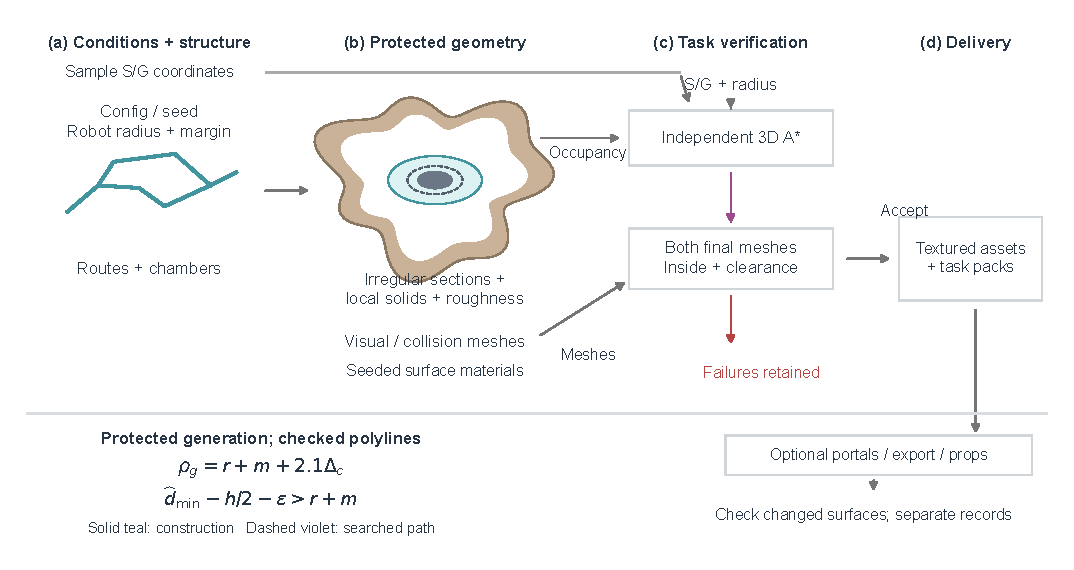
\includegraphics[width=\textwidth]{figures/generated/cave_composer_method.pdf}
\caption{Cave Composer pipeline. Construction routes condition geometry
and endpoint sampling; only occupancy, endpoints and the required radius feed
the independent search. Candidate paths are checked on both final meshes.
Portal/export and post-generation obstacle checks are distinct from the
closed-reference certificate. The lower detail illustrates protection and
the spacing-corrected distance bound. Lines denote construction or geometric
witnesses, not executed robot trajectories.}
\label{fig:method}
\end{figure*}
\subsection{Conditions and intended structure}
A scene request contains structural conditions $c$, a scene seed $s$, and
a spherical robot radius $r$ with margin $m$. The route grammar represents
straight segments, controlled turns and elevation changes, with branches,
rejoining passages and chambers. Later optional sampling presets introduce
curved meanders, dead ends and asymmetric loops. Nominal widths and heights
are controls, not measurements of every local opening. Bounded layout screening
rejects unsuitable route proximity and voxel-budget requests before meshing;
it does not certify the topology of the final free space.

\subsection{Irregular geometry with passage protection}
The generator composes an implicit void field from route-dependent sections
and chambers. Optional morphology controls introduce eccentric section
variation, side cavities, ceiling drops, floor rises, wall intrusions,
overhangs and rockfall-like obstacles. A spatial modulation field changes
roughness across the cave. These mechanisms have separate parameters;
adding uniform high-frequency noise cannot substitute for section asymmetry
or localized solid obstacles.

Let $d_C(x)$ denote the distance approximation to the construction route used
by the generator and $F_{\mathrm{var}}(x)$ its varied void field. Positive field
values denote void. Both terms below are distance-like scalars expressed in
metres, although neither the varied field nor their maximum is an exact SDF.
The maximum is an implementation rule for union of positive regions; acceptance
of the discretized output is determined by final-mesh checks. The rule is
\begin{equation}
\begin{aligned}
F(x)&=\max\{F_{\mathrm{var}}(x),\rho_g-d_C(x)\},\\
\rho_g&=r+m+2.1\Delta_c,
\end{aligned}
\end{equation}
where $\Delta_c$ is the collision-grid spacing. The additional allowance is an
implementation choice for discretization, not a sharp universal error bound.
Final geometric checks remain necessary. The field is not an exact signed
distance function. Surface extraction at separately specified resolutions
produces visual and collision meshes. Their common intended layout does not
make their clearances identical.

\subsection{Independent task search and final-mesh checks}
A task seed selects a fixed budget of start--goal requests within one cave.
The semantic routes may select endpoints, including branch interiors.
The search itself consumes occupancy, grid coordinates, endpoints and the
required radius $\rho=r+m$. It uses a conservative distance transform and
six-neighbor, clearance-weighted A*. No centerline or semantic graph is an
input to this search. Failure under its discretization or search budget does
not prove that all possible continuous paths are infeasible.

For each candidate polyline $P$, samples include its vertices and have maximum
adjacent spacing $h$. On each final mesh $M$, let $d_{\min}(M)$ be the smallest
sampled point-to-triangle distance. Since distance to a fixed surface is
1-Lipschitz, every point of a sampled segment lies within $h/2$ of a sample,
giving the lower bound
\begin{equation}
\inf_{x\in P}d(x,M)\ \geq\ d_{\min}(M)-h/2\ >\ r+m.
\label{eq:clearance}
\end{equation}
Here the analytic bound uses exact distances. The implementation subtracts
an additional tolerance $\epsilon\geq10^{-6}$\,m from computed distances before
testing $\widehat d_{\min}-h/2-\epsilon>r+m$. This is an explicit engineering
allowance, not an interval-arithmetic rounding-error proof. Non-watertight or
inconsistently wound references are rejected before parity is evaluated.
Inside tests assume a valid closed cavity boundary; separate intersection
audits are still needed. Acceptance
requires both visual and collision checks. The bound applies to a spherical
static envelope and does not certify dynamics, tracking error or perception.
Each request retains its outcome; failed tasks are not replaced to inflate
the accepted fraction.

\subsection{Exports, appearance and modified surfaces}
Materials use a separate appearance seed. Optional reviewed scan-color patches
have source-group records; they do not establish a fitted geometric prior or
recover physical reflectance. Portable texture exports retain the association
between geometry, material and hashes.

Portal cutting is a separate deterministic export from a closed reference.
The procedural portal checker requires two intentional boundary loops and
tests a crossing path against the resulting open surfaces. Portable-format
checks inspect reimported geometry and coordinates. Showcase obstacles have
their own combined-surface checks. These records are scoped to the path they
actually check. The current portal exporter reuses the independently searched
interior path and adds separately checked straight terminal approaches.
An open export uses unsigned triangle distance, never an open-mesh parity
result. Fresh delivery checks reload both OBJs, merge only exactly coincident
UV-seam vertices without changing triangles, and bind certificates to file
and path hashes. A closed certificate must never silently
carry over to a changed collision mesh, added obstruction or simulator import.
Arbitrary simulator conversion currently requires an additional runtime gate.

\subsection{Reproducibility and geometric evaluation}
Scene and task records include seeds, normalized configuration, file hashes,
code-file hashes, dependency identity and retained failures. The package
version label alone is insufficient: multiple later updates still use the
same version string. Dataset manifests must therefore identify the exact
generator sources that produced their assets.

A local integrity audit recovered 36 accepted task records on three historical
caves, with 12 requested tasks per cave. A separate, later morphology snapshot
contains six checked configurations at one shared scene seed. These are
different versioned evidence sets, not a single benchmark or 36 independent
caves. Integrity replay checks persisted records; it is not a new policy
experiment or a fresh distance computation. The new paired pilot below is a
separate evidence set with fresh checks of delivered geometry.
